\documentclass[10pt]{article}
\usepackage[polish]{babel}
\usepackage[utf8]{inputenc}
\usepackage[T1]{fontenc}
\usepackage{graphicx}
\usepackage[export]{adjustbox}
\graphicspath{ {./images/} }
\usepackage{amsmath}
\usepackage{amsfonts}
\usepackage{amssymb}
\usepackage[version=4]{mhchem}
\usepackage{stmaryrd}

\title{LIGA MATEMATYCZNA im. Zdzisława Matuskiego GRUDZIEŃ 2018 SZKOŁA PODSTAWOWA }

\author{}
\date{}


\begin{document}
\maketitle
(klasy IV - VI)

\section*{ZADANIE 1.}
Na każdej ściance sześciennej kostki napisano dodatnią liczbę całkowitą. Iloczyn liczb na przeciwległych ściankach jest taki sam dla każdej pary takich ścianek. Napisane liczby nie muszą być różne. Jaka jest najmniejsza możliwa suma wszystkich liczb znajdujących się na kostce?\\
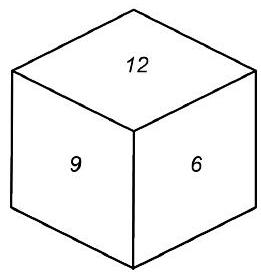
\includegraphics[max width=\textwidth, center]{2024_11_21_a81a4da0f1de819f5471g-1}

\section*{ZADANIE 2.}
Babcia upiekła na święta Bożego Narodzenia 1000 pierników. Wnuki Ania i Bartek bawią się w następujacą grę: w każdym ruchu zabierają z koszyka połowę pierników, jeżeli ich liczba jest parzysta lub jedno ciastko, jeżeli liczba pierników jest nieparzysta. Po ilu ruchach wyjmą wszystkie pierniki z koszyka?

\section*{ZADANIE 3.}
W Wigilię bracia Adam, Bartek i Czarek zjedli półmisek pierogów. Adam zjadł o 6 pierogów mniej niż Bartek, Bartek zjadł dwa razy więcej pierogów niż Czarek, a Czarek o 2 więcej niż Adam. Ile pierogów zjedli chłopcy?

\section*{ZADANIE 4.}
Dodając 9 jednakowych liczb dwucyfrowych oraz jedną liczbę jednocyfrową Mikołaj otrzymał 257. Znajdź liczbę jednocyfrową.

\section*{ZADANIE 5.}
Dane są dwa okręgi o środkach \(O_{1}, O_{2}\) styczne zewnętrznie, każdy o promieniu 3. Prosta \(p\) równoległa do prostej \(\operatorname{pr}\left(O_{1}, O_{2}\right)\) przecina te okregi w punktach \(A, B, C, D\) tak, jak na rysunku. Odcinek \(B C\) ma długość 2. Oblicz długość odcinka \(A D\).\\
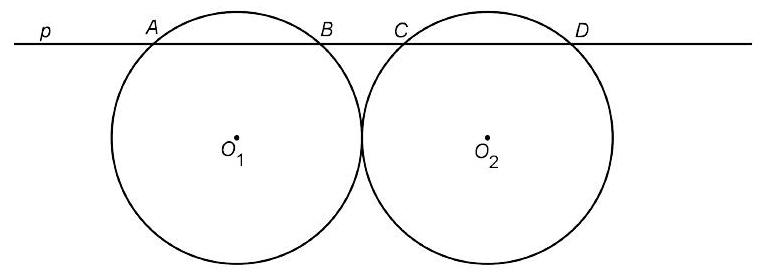
\includegraphics[max width=\textwidth, center]{2024_11_21_a81a4da0f1de819f5471g-1(1)}


\end{document}